\documentclass{article}
\usepackage{importer}
\usepackage[backend=biber]{biblatex}
\addbibresource{kilder.bib}

\title{Faste Stoffers Fysikk: Løsningsforslag til øvinger}
\author{Sebastian Siljuholtet Johansen}
\date{Vår 2024}

\begin{document}

\maketitle

\newpage
\section*{Ingress}
Skrevet av studenter. Notater er tatt under forelesningene i TFY4220 Faste Stoffers Fysikk av Dag Werner Breiby og er veldig basert på boken Introduction to Solid State Physics av C. Kittel. Øvingene er løst av Sebastian Siljuholtet Johansen.

\newpage
\tableofcontents

\newpage
\oving{1}
\oppgave{1}
\deloppgave{a}
Hva er den mattematiske definisjonen til en krystall? Vel, man kan definere en krystall som et periodisk gitter med ulike symmetrier knyttet til ethvert krystall. Krystallene er videre bygget opp av en basis knyttet til hvert gitter som er knyttet til hvilke atomer som er plassert hvor og koblet til hvilke andre atomer. Matematisk blir da krystallen konvolusjonen av gitteret med basisen.

Altså blir en krystall en periodisk struktur av bygningsblokker. Disse bygningsblokkene kan være atomer, parr med atomer, komplekse molekyler eller liknende.

Vi skriver mattematisk derfor fra over at:
\begin{equation}
    C(x) = \underbrace{G(x)}_{\text{gitterstrukturen}}\otimes \underbrace{B(x)}_{\text{basisen}}
\end{equation}
\deloppgave{b}
Et primitivt gitter i tre dimensjoner er definert av tre vektorer $\vec{a}_1, \vec{a}_2$ og $\vec{a}_3$ slik at enhver vektor mellom gitterpunkt $\Vec{T}$ kan bli beskrevet som:
\begin{equation}
    \vec{T} = u_1 \vec{a}_1+ u_2 \Vec{a}_2 +  u_3 \Vec{a}_3
\end{equation}
hvor $u_1, u_2$ og $u_3$ er vilkårlige heltall. 
\deloppgave{c}
Den primitive Wigner-Seitz-cellen er definert gjennom å lage linjer mellom alle de nærmest gitterpunktene og deretter lage tversgående plan halvveis på midten av alle disse. Det minste volumet som skapes av disse planene er da Wigner-Seitz-cellen.
\deloppgave{d}
En trefoldig rotasjon er en rotasjon på 120 grader. En n-foldig rotasjon er en rotasjon på $\frac{360}{n}$ grader. Hvis noe er invariant under en slik rotasjon vil den være lik på 
\oppgave{2}
\deloppgave{a}
Bikakegitteret er ikke et primitivt gitter fordi det finnes to forskjellige typer punkter i det. Altså har vi ikke bare samme type gitterpunkt. Derfor må bikakegitteret bestå av en basis av to atomer og et primitivt gitter i bakgrunnen. En illustrasjon av de ulike typene er de blå og rød atomene her:
\begin{figure}[H]
    \centering
    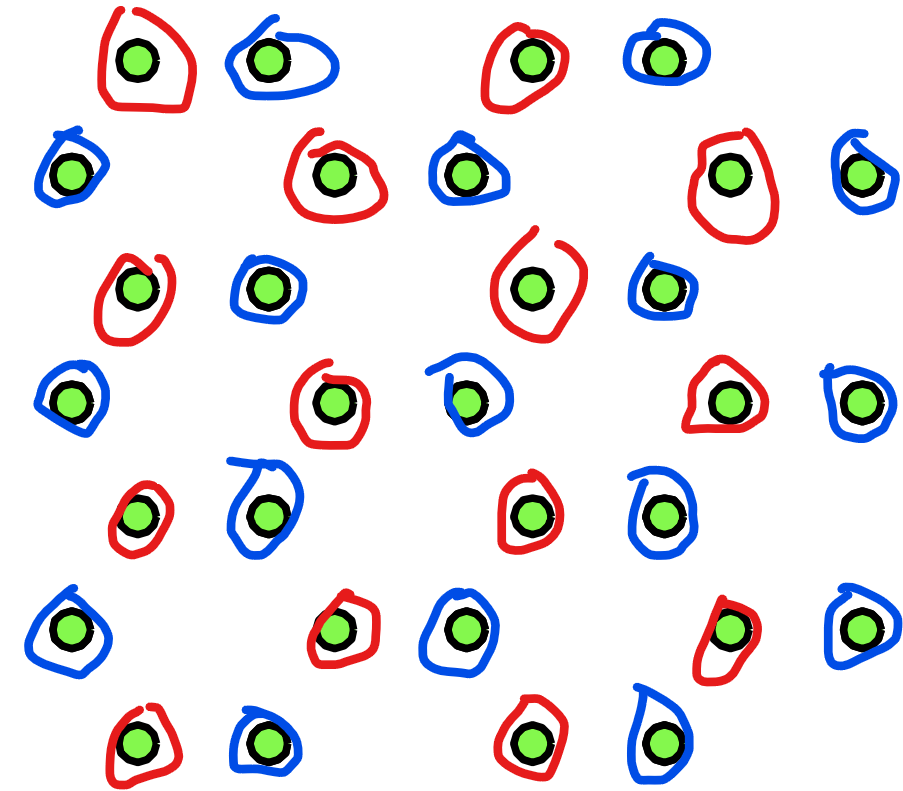
\includegraphics[width=0.2\linewidth]{bilder_lf/bikake_gitterstruktur.png}
    \caption{Strukturen i bikakegitteret}
    \label{fig:bikake_gitterstruktur}
\end{figure}
Her må basisen bestå av et rødt og et blått atom. Videre må det primitive gitteret bestå av kun en av fargene. Dette Bravaisgitteret må være et skrått rektangulært mønster.
\deloppgave{b}
Et Bravais-gitter kan bli beskrevet på to måter:
\begin{itemize}
    \item En uendelig mengde med diskré punkter som er arrangert på en måte som ser likt ut uansett hvor du er og hvordan orientasjonen er.
    \item Alle punkter som er beskrevet på formen: $\vec{R}_{mno} = m \vec{a} + n\vec{b} + o\vec{c}$ hvor $m, n$ og $o$ er heltall og vektorene er vilkårlige. Her må også vektorene være lineært uavhengige og dermed ikke i samme plan eller linje. 
\end{itemize}
\deloppgave{c}
Flere forskjellige typer enhetsceller vi kan velge her er de som er i bildet under:
\begin{figure}[H]
    \centering
    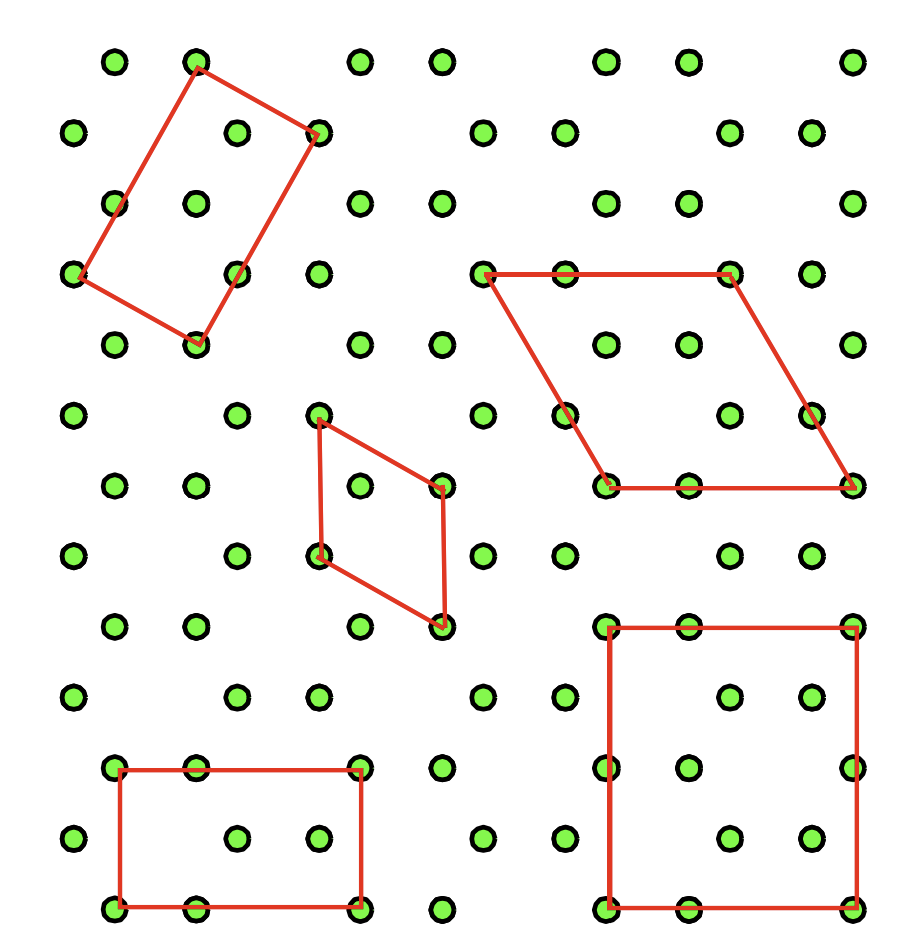
\includegraphics[width=0.25\linewidth]{bilder_lf/typer_enhetsceller_i_bikakegitteret.png}
    \label{fig:typer_enhetsceller_i_bikakegitteret}
    \caption{Noen enhetsceller i bikakegitteret}
\end{figure}
Den mest normale typen enhetscelle er den definert på måten beskrevet i deloppgave a). Her har vi at strukturen blir heksagonal med to atomer i basisen hvor vinkelen mellom vektorene som beskriver Bravais-gitteret blir 120 grader. Dette blir da enten det røde eller det røde gitteret i figuren fra deloppgave a) (\ref{fig:bikake_gitterstruktur})
\oppgave{3}
\deloppgave{a}
\begin{enumerate}
    \item For en romsentrert kubisk (B.C.C) struktur med sfærer, vil vi få en sfære på hvert gitterpunkt. ALtså en kube med sfærer på hvert hjørne og en i midten. Vi antar at kuben har sidekanter med lengde 1. Da må sfærene ha radius 0.5. Derimot gjør sfæren i midten at vi må ha en radius som tilsvarer at 4 radiuser (en fra to hjørner og to fra midten) går over diagonalen som får lengde $\sqrt{3}$. Altså blir radiusen til sfærene $\frac{\sqrt{3}}{4} = \frac{1}{2 \sqrt{2}}$. Volumet til disse sfærene vil bli det samme som 8 sfærer med bare en åttendedel fra hver og hele den i midten. Altså totalt to sfærer med den radiusen. De får volum: $V = 2 * 4 \pi \left(\frac{\sqrt{3}}{4}\right)^3 / 3 = \frac{\pi \sqrt{3} 3}{24} = 0.68017476158$. Altså blir pakkeprosenten på $68.0174\%$
    \item For en FCC-pakket sfære må vi først se på sidene. Her får vi 9 sfærer som vi kan identifisere på hver side. Dette vil gi oss at den aller høyeste radiusen vi kan få på sideflatene er $1/4$ av diagonalen på en flate. Altså $\sqrt{2} / 4$. siden vi kan ha 4 radiusen totalt over en sideflate. Da vil vi få 1 sfære siden vi ikke har noen i midten nå. Sideflatene gir oss 3 sfærer til. Altså får vi et totalt volum: $V = 4 * 4 * \pi \left(\frac{\sqrt{2}}{4}\right)^3 / 3 = 2 \sqrt{2} \pi / 12 = 0.74048048969$ som gir oss en pakkeprosent på $74.048\%$.
\end{enumerate}
\deloppgave{b}
Forholdet her blir:
\begin{align}
    \frac{\Phi_{f.c.c}}{\Phi_{b.c.c}}\frac{\frac{\pi \sqrt{3} 3}{24}}{2 \sqrt{2} \pi / 12} = \frac{3}{4} \sqrt{\frac{3}{2}} = 0.91855865354
\end{align}
\oppgave{4}
\deloppgave{a}
\begin{enumerate}
    \item Her vil vi få indeksene $(hkl) = (\bar{1}21)$ siden forholdene er inversen av disse.
    \item Her vil få få indeksene $(hkl) = (0\bar{2}0)$ siden $1/|a_1| = 1/|a_3| = 1 / \infty$, mens $1 / |a_2| = 1 / (- 1/2) = -2$.
\end{enumerate}
\deloppgave{b}
Et generelt plan med (hkl) indekser kan bli tegnet på følgende måte (\ref{fig:hkl_plan}):
\begin{figure}[H]
    \centering
    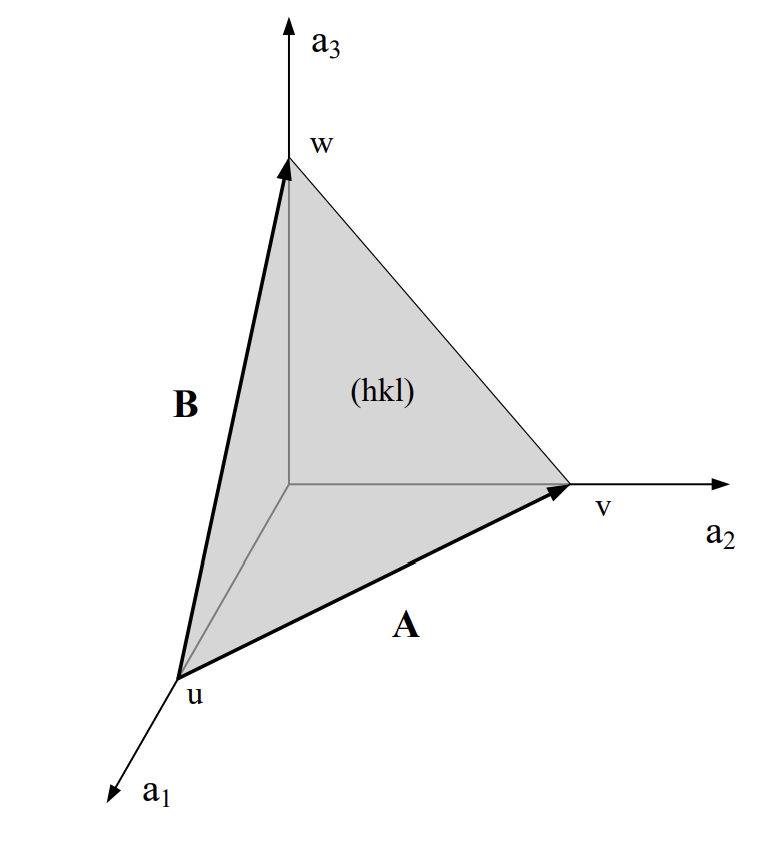
\includegraphics[width=0.5\linewidth]{bilder_lf/hkl_plan.png}
    \caption{Generelt (hkl) plan}
    \label{fig:hkl_plan}
\end{figure}
Her kan vektorene A og B spenne planet. Disse er definert som:
\begin{align}
    \vec{A} = -u \vec{a}_1 + v\vec{a_2}\\
    \vec{B} = -u \vec{a}_1 + w\vec{a_3}
\end{align}
Normalvektoren til dette planet er kryssproduktet til disse vektorene. Dette blir som følger:
\begin{align}
    \vec{A} \times \vec{B} = uvw( \frac{1}{u} \vec{a}_1+\frac{1}{v} \vec{a}_2+\frac{1}{w} \vec{a}_3)
\end{align}
Inversen av disse lengdene er jo $hkl$ lengdene våre multiplisert med en konstant. Altså har vi at:
\begin{align}
    \vec{A} \times \vec{B} &= uvw( \frac{1}{u} \vec{a}_1+\frac{1}{v} \vec{a}_2+\frac{1}{w} \vec{a}_3) \\
    &= uvw( Kh \vec{a}_1+Kk \vec{a}_2+Kl \vec{a}_3)\\
    &= uvw K\underbrace{( h \vec{a}_1+k \vec{a}_2+l \vec{a}_3)}
\end{align}
Og dermed ser vi at vektoren som har parantes under seg. Denne vektoren er jo vektoren i retningen (hkl). Altså må planet i seg selv være ortogonalt med denne vektoren siden planets normalvektor er parallelt med den retningen.
\deloppgave{c}
Den normaliserte normalvektoren vår i dette tilfellet blir:
\begin{equation}
    \vec{n}= \frac{ \vec{A} \times \vec{B}}{| \vec{A} \times \vec{B}|} = \frac{1}{a} \frac{( h \vec{a}_1+k \vec{a}_2+l \vec{a}_3)}{\sqrt{h^2 + k^2 + l^2}}
\end{equation}
Planene vil bli en forskyvning langs aksene med en lengde 1. Altså vil vi finne lengden mellom planene til å være en translasjon langs en av aksene prosjektert på  normalvektoren. Da vil få få:
\begin{align}
    d_{hkl} &= \frac{\vec{a}_i \cdot \vec{n}}{(h, k, l)} \\
    &= \frac{1}{(h, k, l)} \frac{(h, k, l) |\vec{a}_i|^2}{a \sqrt{h^2 + k^2 + l^2}} \\
    &= \frac{a^2}{a\sqrt{h^2 + k^2 + l^2}} \\
    &= \frac{a}{\sqrt{h^2 + k^2 + l^2}}
\end{align}
\deloppgave{d}
Tettpakningen i FCC krever følgende bilde:
\begin{figure}[H]
    \centering
    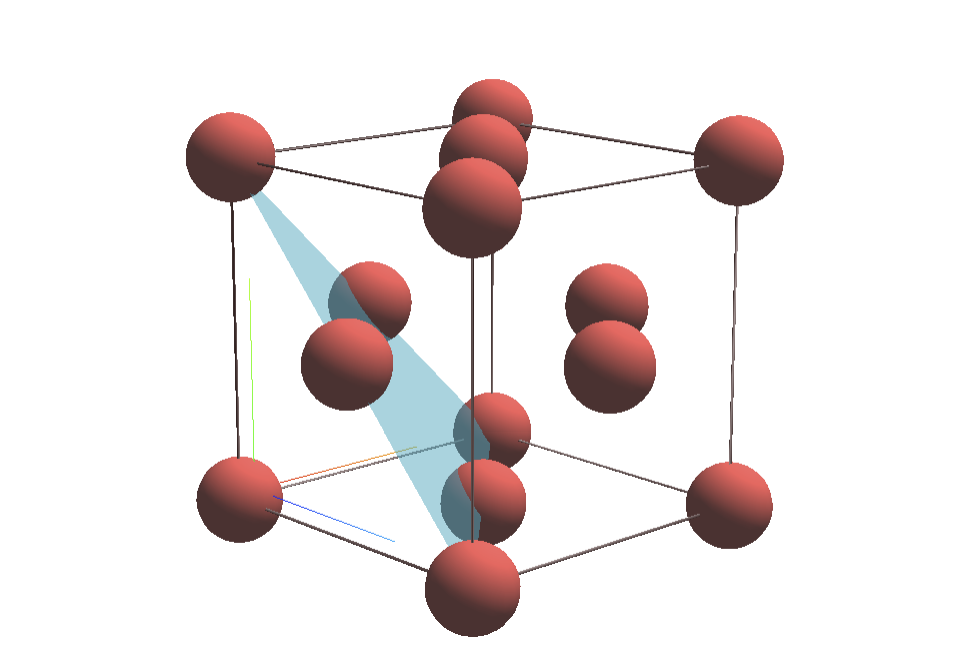
\includegraphics[width=0.5\linewidth]{bilder_lf/tettpakning_fcc.png}
    \caption{Plan FCC}
    \label{fig:tettpakning_fcc}
\end{figure}
Her har vi ikke tegnet et tettpakket gitter, men man kan se hvilket plan som må til for å få FCC-gitteret. Dette planet er da (111) planet.
På samme måte kan vi se hvilket plan som må til for BCC gitteret. Her blir det igjen noe tegnet som:
\begin{figure}[H]
    \centering
    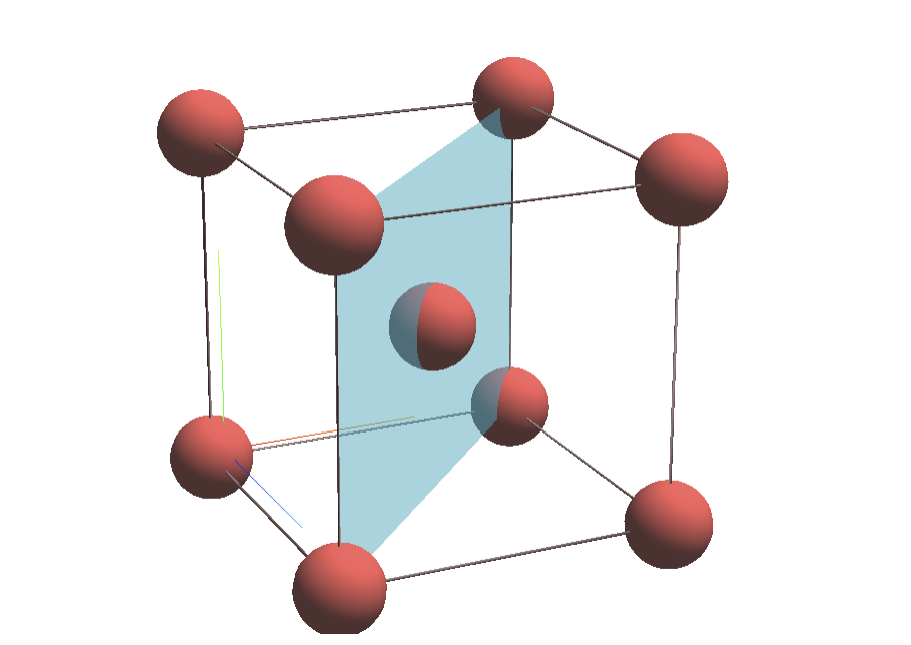
\includegraphics[width=0.5\linewidth]{bilder_lf/tettpakket_bcc.png}
    \caption{Plan BCC}
    \label{tettpakket_bcc}
\end{figure}
som gir oss planet (110).

I begge bildene over er origo nederst til venstre.
\nyside
\oving{2}
\oppgave{1}
\deloppgave{a}
\deloppgave{b}
\deloppgave{c}
\deloppgave{d}
\deloppgave{e}
\oppgave{2}
\deloppgave{a}
\deloppgave{b}
\deloppgave{c}
\deloppgave{d}
\oppgave{3}
\nyside
\oving{3}
\nyside
\oving{4}
\nyside
\oving{5}
\nyside
\oving{6}
\nyside
\oving{7}
\nyside
\oving{8}
\nyside
\oving{9}
\nyside
\oving{10}
\nyside
\oving{11}
\newpage
\printbibliography
\end{document}